% ------------------------------------------------------------------------------
% Este fichero es parte de la plantilla LaTeX para la realización de Proyectos
% Final de Grado, protegido bajo los términos de la licencia GFDL.
% Para más información, la licencia completa viene incluida en el
% fichero fdl-1.3.tex

% Copyright (C) 2012 SPI-FM. Universidad de Cádiz
% ------------------------------------------------------------------------------

%En esta sección se recoge la arquitectura general del sistema de información, la parametrización del software base (opcional), el diseño físico de datos, el diseño detallado de componentes software y el diseño detallado de la interfaz de usuario.
En esta sección se recoge la arquitectura general del sistema de información, la parametrización del software base, el diseño físico de datos, el diseño detallado de componentes software y el diseño detallado de la interfaz de usuario.

%5.1
\section{Arquitectura del Sistema}
%En esta sección se define la arquitectura general del sistema de información, especificando la infraestructura tecnológica necesaria para dar soporte al software y la estructura de los componentes que lo forman.
En esta sección definiremos la arquitectura general del sistema de información, especificando la infraestructura tecnológica necesaria para dar soporte al software y la estructura de los componentes que lo forman.


%5.1.1
\subsection{Arquitectura Física}
%En este apartado, describimos los principales elementos hardware que forman la arquitectura física de nuestro sistema, recogiendo por un lado los componentes del entorno de producción y los componentes de cliente.\\

%Se debe incluir un modelo de despliegue en el cual se describe cómo los elementos software son desplegados en los elementos hardware. También se incluyen las especificaciones y los requisitos del hardware (servidores, etc.), así como de los elementos software (sistemas operativos, servicios, aplicaciones, etc.) necesarios.
Los componentes que compondrán la arquitectura física de esta aplicación se puede ver reflejado en las figura \ref{fig:arquitectura-fisica01} y \ref{fig:arquitectura-fisica02}.

\begin{itemize}
	\item \textbf{Navegador del cliente}. Un navegador estándar HTML capaz de soportar  CSS, Javascript + Document Object Model, XML y XSLT. Este servirá como dispositivo de interfaz de usuario. Toda la interacción entre los usuarios y el sistema se realiza a través del navegador.
	\item \textbf{Servidor web}. El navegador del cliente accederá al sistema a través del servidor Web (Tomcat), el cual acepta las peticiones del cliente y ejecuta, tosi es necesario, los scripts del lado del servidor necesarios. El resultado, una página HTML formateada, será enviada al cliente.
	\item \textbf{Conexión HTTP}. Es el protocolo más común actualmente entre el cliente y el servidor.
	\item \textbf{Servidor de Aplicaciones}. Es el principal motor para ejecutar la lógica del negocio del lado del servidor.
	\item \textbf{Servidor de Base de datos}. Es la parte del sistema que mantiene el estado actual del negocio.
	\item \textbf{Servicio Web}. En este caso, Mendeley actuará de gestor de referencias del cuál podremos obtener la información de las revisiones sistemáticas (carpetas), ficheros (referencias) e información del perfil del usuario.
\end{itemize}

\begin{figure}[!hp]
	\begin{center} 
		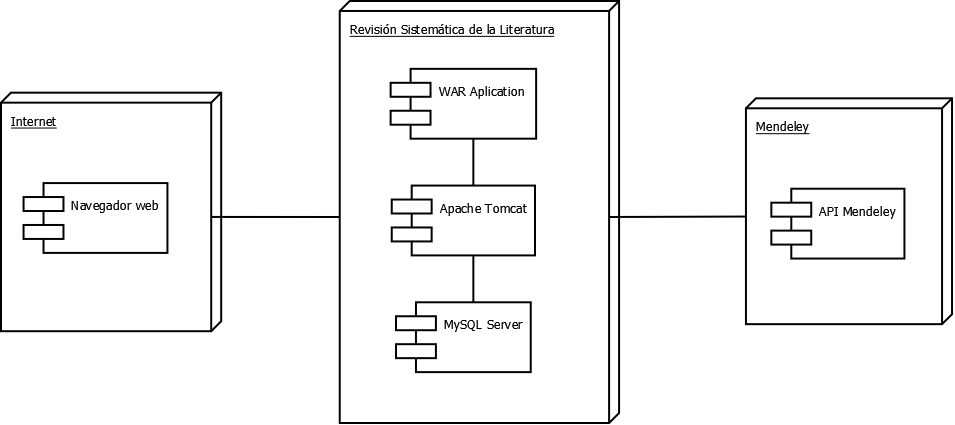
\includegraphics[scale=0.3]{arquitectura-fisica.png}
		\caption{Arquitectura física del sistema (I).}
		\label{fig:arquitectura-fisica01}
	\end{center}
\end{figure}

\begin{figure}[!hp]
	\begin{center} 
		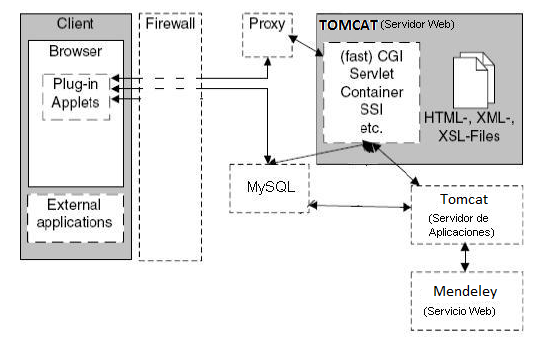
\includegraphics[scale=0.9]{arquitectura-fisica2.png}
		\caption{Arquitectura del sistema (II).}
		\label{fig:arquitectura-fisica02}
	\end{center}
\end{figure}

El servidor tiene las características descritas en la tabla \ref{table:arqui-server}. En él, se ha instalado Tomcat, Apache y MySQL para la base de datos.

\begin{table}[!hbt]
	\begin{center}
		\begin{tabular}{|p{4cm}|p{11cm}|}
			\hline
			\textbf{CPU} & 1vCore\\
			\hline
			\textbf{RAM} & 2048 MB.\\
			\hline
			\textbf{Storage} & 40 GB SSD.\\
			\hline
			\textbf{Bandwidth} & 2000 GB\\
			\hline
		\end{tabular}
		\caption{Arquitectura del Servidor}
		\label{table:arqui-server}
	\end{center}
\end{table}

%5.1.2
\subsection{Arquitectura Lógica}
%La arquitectura de diseño especifica la forma en que los artefactos software interactúan entre sí para lograr el comportamiento deseado en el sistema. En esta sección se muestra la comunicación entre el software base seleccionado, los componentes reutilizados y los componentes desarrollados para cumplir los requisitos de la aplicación. También, se recogen los servicios de sistemas externos con los que interactúa nuestro sistema.
%Se debe incluir un diagrama de componentes que muestre en un alto nivel de abstracción los artefactos que conforman el sistema.\\

%Existen diferentes patrones o estilos arquitectónicos. En los sistemas web de información es común la utilización del patrón Layers (Capas), con el cual estructuramos el sistema en un número apropiado de capas, de forma que todos los componentes de una misma capa trabajan en el mismo nivel de abstracción y los servicios proporcionados por la capa superior utilizan internamente los servicios proporcionados por la capa inmediatamente inferior. Habitualmente se tienen las siguientes capas:

La arquitectura lógica de la aplicación web se va a regir en todo momento según el patrón \textbf{Modelo Vista Controlador} (\textbf{MVC}). Éste separa los datos de la planificación, la interfaz del usuario y la lógica de control o negocio en tres modelos distintos.

\begin{itemize}
	\item \textbf{Capas de datos}. Contiene los componentes que representan y gestionan los datos manejados por la aplicación. En el caso más típico, los objetos encargados de leer y escribir en base de datos.
	\item \textbf{Capa de presentación}. Los componentes de esta capa son responsables de mostrar al usuario el estado actual del modelo de datos, y presentarle las distintas acciones disponibles.
	\item \textbf{Capa de control}. Contendrá todos los componentes que reciban las órdenes del usuario, gestionan la aplicación de la lógica de negocio sobre el modelo de datos, y determinan qué vista debe mostrarse a continuación.
	\item \textbf{Capa de servicios}. Se trata de una cuarta capa que contiene los elementos encargados de implementar la lógica de negocio de nuestra aplicación.
\end{itemize}

Para el desarrollo de la aplicación, se ha decidido seguir la arquitectura del framework \textbf{Grails} (ver figura \ref{fig:arquitectura-grails}) que acopla correctamente el patrón MVC \cite{brito2009}.

\begin{figure}[!hp]
	\begin{center} 
		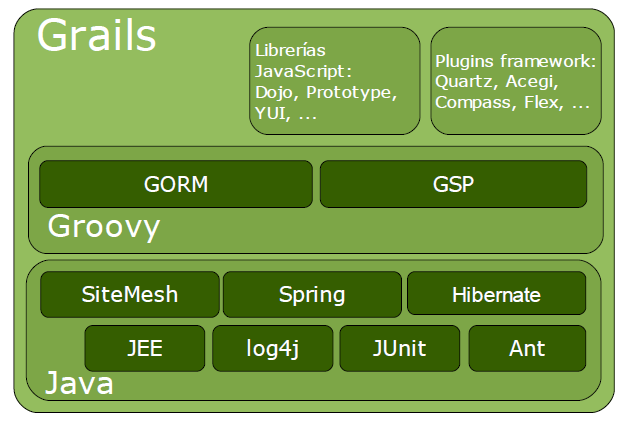
\includegraphics[scale=0.7]{arquitectura-grails.png}
		\caption{Arquitectura Grails.}
		\label{fig:arquitectura-grails}
	\end{center}
\end{figure}

\begin{itemize}
	\item \textbf{Modelo}. Es la representación específica de la información con la cual el sistema opera. La lógica de datos asegura la integridad de éstos. El SGBD para gestionar los datos corresponde a este componente. En este sistema el mapeo se realiza a través de \textbf{GORM} (\textit{Grails Object-Relational Mapping}) que a través de clases escritas en \textbf{Groovy} describe todo el modelo de la aplicación.
	\item \textbf{Vista}. Presenta el modelo en un formato adecuado para interactuar, normalmente la interfaz de usuario. La vista estará formada por un conjunto de páginas webs que facilitaran al usuario la interacción con el sistema. Las páginas se renderizan a partir de ficheros fuentes GSP (Groovy Server Pages) que mezcla etiquetas HTML con otras propias de Grails.
	\item \textbf{Controlador}. Responde a los eventos, generalmente provocados por el usuario a través de las vistas, ajustando los modelos. Estos controladores serán clases escritas en Groovy con cada una de las acciones posibles.
\end{itemize}

Grails es un framework para desarrollo de aplicaciones web construido sobre cinco fuertes pilares:

\begin{itemize}
	\item Groovy. Para la creación de propiedades y métodos dinámicos en los objetos de la aplicación.
	\item Spring. Para los flujos de trabajo e inyección de dependencias.
	\item Hibernate. Para la persistencia de los datos de la aplicación.
	\item SiteMesh. Para la composición de la vista.
	\item Ant. Para la gestión del proceso de desarrollo.
\end{itemize}

La estructura de esta aplicación será la siguiente:

\begin{itemize}
	\item grails-app
\begin{itemize}
	\item conf: Archivos de configuración.
	\item hibernate: Configuración de Hibernate.
	\item spring: Configuración de Spring.
	\item controllers: Controladores.
	\item domain: Entidades (Clases de Dominio).
	\item i18n: Message Bundles.
	\item services: Servicios.
	\item taglib: Librerías de etiquetas.
	\item util: Clases de utilidad.
	\item views: Vistas.
	\item layouts: Layouts SiteMesh.
	\item lib
	\item scripts
	\item src
	\begin{itemize}
		\item groovy: Clases Groovy.
		\item java: Clases Java.
	\end{itemize}
	\item test: Casos de prueba.
	\item web-app: Raíz de la aplicación web.
	\end{itemize}
\end{itemize}

%\paragraph*{Capa de presentación (frontend)}
%Este grupo de artefactos software conforman la capa de presentación del sistema, incluyendo tanto los componentes de la vista como los elementos de control de la misma.

%\paragraph*{Capa de negocio}
%Este grupo de artefactos software conforman la capa de negocio del sistema, incluyendo los elementos del modelo de dominio y los servicios (operaciones del sistema).

%\paragraph*{Capa de persistencia}
%Este grupo de artefactos software conforman la capa de integración del sistema, incluyendo las clases de abstracción para el acceso a datos (BD o sistema de ficheros) o a sistemas heredados.\\

%Es común que a la capa de negocio y de datos de los sistemas web, se denomine conjuntamente como backend o modelo de la aplicación.

%Opcionalmente, podemos disponer de un conjunto de artefactos software que pueden ser usados por elementos de cualquiera de las capas del sistema y que fundamentalmente proporcionan servicios relacionados con requisitos no funcionales (calidad).

%5.2
\section{Parametrización del software base}
%En esta sección, se detallan las modificaciones a realizar sobre el software base, que son requeridas para la correcta construcción del sistema. En esta sección incluiremos las  actuaciones necesarias sobre la interfaz de administración del sistema, sobre el código fuente o sobre el modelo de datos.
Esta aplicación hace conexión a través de una API al gestor de referencias Mendeley. Para realizar este proceso, se necesita un usuario que actue como administrador del sistema y que se conecte con sus datos al portal de Mendeley para indicar que esta aplicación pueda tener conexión con Mendeley.\\

Mendeley, dispone de una sección donde todos los usuarios pueden insertar la configuración necesaria para que Mendeley conecte con sus aplicaciones. Para ello, es necesario dirigirse a \url{http://dev.mendeley.com/} y a continuación elegir la opción \textit{My Apps}.\\

Una vez que se ha logado en el sistema, podemos obtener un listado de aplicaciones (ver figura \ref{fig:mend-register}) con todas las aplicaciones que un usuario disponga. Mendeley pide por pantalla varios datos de configuración, pero es necesario recordar tres campos que serán necesarios para la configuración en nuestra aplicación como describiremos más adelante (marcados en negrita). Como podemos comprobar, se puede tener tantas configuraciones como se desee. Ésto podrá ser válido si, por ejemplo, tuviésemos varios entornos de desarrollo.

\begin{itemize}
	\item Application name. Nombre de la aplicación.
	\item Description. Descripción de lo que realiza esta aplicación.
	\item \textbf{ID Cliente}. Identificador de esta aplicación en Mendeley. Es generado automáticamente por Mendeley.
	\item \textbf{Redirect URL}. Esta aplicación hará conexión con Mendeley a través de OAuth2, donde se nos pedirá unos datos que enviarán a una página de nuestra aplicación. 
	\item \textbf{Client Secret}. Código privado del cliente que debe ser generado a través del botón \textit{Generate secret}.
\end{itemize}

\begin{figure}[!hp]
	\begin{center} 
		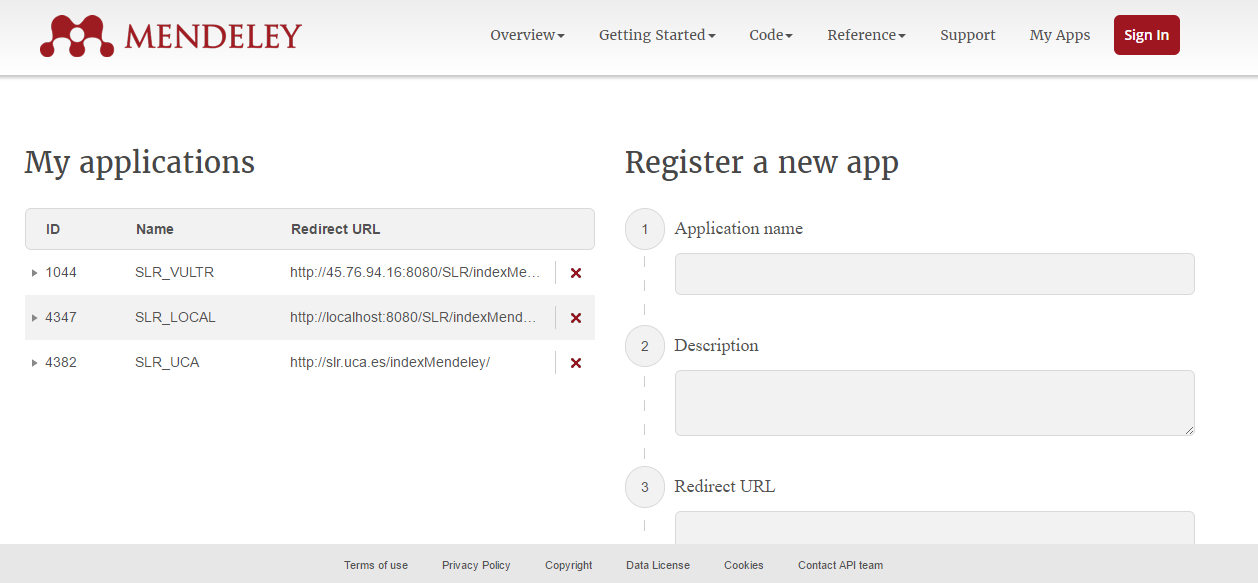
\includegraphics[scale=0.4]{mendeley-registerApp.png}
		\caption{Registrar aplicación en Mendeley.}
		\label{fig:mend-register}
	\end{center}
\end{figure}

Una vez que hemos realizado la configuración en Mendeley, debemos insertar la información obtenida en nuestra aplicación. Para ello, Grails dispone de un fichero situado en \textit{conf/Bootstrap.groovy} donde por medio de una clase de dominio realizada denominada \textit{MendeleyApi} podemos parametrizar esta configuración tal y como podemos ver reflejado en la figura \ref{fig:bootstrap-mend}.

\begin{figure}[!hp]
	\begin{center} 
		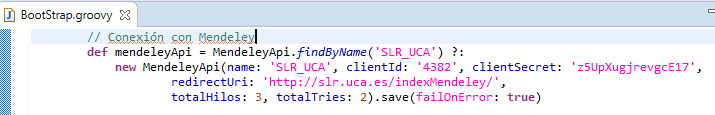
\includegraphics[scale=0.6]{bootstrap-mend.png}
		\caption{Registrar aplicación en Mendeley.}
		\label{fig:bootstrap-mend}
	\end{center}
\end{figure}

Si la aplicación se encuentra desplegada sobre el servidor, y siempre siendo administrador, podemos modificar esta configuración a través de un menú que dispone un usuario con este rol.

%5.3
\section{Diseño Físico de Datos}
En esta sección se define la estructura física de datos que utilizará el sistema, a partir del modelo de conceptual de clases, de manera que teniendo presente los requisitos establecidos para el sistema de información y las particularidades del entorno tecnológico, se consiga un acceso eficiente de los datos.
La estructura física se compone de tablas, índices, procedimientos almacenados, secuencias y otros elementos dependientes del SGBD a utilizar.

%5.4
\section{Diseño detallado de Componentes}
Para cada uno de los módulos funcionales del sistema debemos realizar un diagrama de secuencia, para definir la interacción existente entre las clases de objetos que permitan responder a eventos externos.

%5.5
\section{Diseño detallado de la Interfaz de Usuario} 
En esta sección se detallarán las interfaces entre el sistema y el usuario, incluyendo un prototipo de alta fidelidad con el diseño de la IU. Se definirá el comportamiento de las diferentes pantallas, indicando qué ocurre en los distintos componentes visuales de la interfaz cuando aparecen y qué acciones se disparan cuando el usuario trabaja con ellas.

